\documentclass[12pt,a4]{article}
\usepackage[english]{babel}
\usepackage[utf8]{inputenc}
\usepackage[T1]{fontenc}
\usepackage{geometry}
\usepackage{float}
\geometry{
	a4paper,
	left=20mm,
	right=20mm,
	top=20mm,
	bottom=20mm,
}
% Useful packages
\usepackage{amsmath}
\usepackage{bm}
\usepackage{graphicx}
\usepackage[colorlinks=true, allcolors=blue]{hyperref}

\begin{document}

\section{Modelling}


\subsection{Kinematics}
The dynamic of a vessel can be described as follows, using a 6 DOF model.
\begin{align}
	\bm{M}_{RB}\bm{\dot{\nu}} + \bm{M}_{A}\bm{\dot{\nu_r}} + \bm{C}_{A}(\bm{\nu})\bm{\nu} + \bm{C}_{RB}(\bm{\nu}_r)\bm{\nu}_r
	+ \bm{D}(\bm{\nu}_r)\bm{\nu}_r +\bm{G}\bm{\eta} & = \bm{\tau} + \bm{w}(t) \\
	\bm{\dot{\eta}}                                 & = \bm{J}(\eta)\bm{\nu}
\end{align}
where $\nu$ is the velocities and $\eta$ is the positions. This description includes a velocity and a position in each of the 6 modes.
The modes are translation in x, y and z and rotation around x, y and z. $\nu_r$ is the relative speed of the vessel to the water

\subsection{State space}
Assuming $\nu = \nu_r$ (no movement of the water relative to the seabed), we can define

\begin{align}
	\bm{M}           & = \bm{M}_{RB} + \bm{M}_{A}                     \\
	\bm{C}(\bm{\nu}) & = \bm{C}_{RB}(\bm{\nu}) + \bm{C}_{A}(\bm{\nu})
\end{align}
And write the system as
\begin{align}
	\bm{M}\bm{\dot{\nu}} + \bm{C}(\bm{\nu})\bm{\nu} + \bm{D}(\bm{\nu})\bm{\nu} +\bm{G}\bm{\eta} & = \bm{\tau} + \bm{w}(t) \\
	\bm{\dot{\eta}}                                                                             & = \bm{J}(\eta)\bm{\nu}
\end{align}
Solving for $\bm{\dot{\nu}}$ we get
\begin{align}
	\bm{\dot{\nu}}  & =	\bm{A}(\bm{\nu})\bm{\nu}+\bm{G}\bm{\eta}+\bm{B}\bm{\tau} 		\label{eq:nu_ss} \\
	\bm{\dot{\eta}} & =	\bm{J}(\eta)\bm{\nu}								\label{eq:eta_ss}
\end{align}
Where
\begin{align}
	\bm{A}(\bm{\nu}) & = -\bm{M}^{-1}(\bm{C}(\bm{\nu})+\bm{D}(\bm{\nu})) \\
	\bm{B}           & = \bm{M}^{-1}
\end{align}
Writing (\ref{eq:nu_ss}) and (\ref{eq:eta_ss}) in matrix form gives us a state space description of the whole system

\begin{equation}
	\bm{\dot{x}} =	\begin{bmatrix} \bm{A} & \bm{G} \\ \bm{J}(\eta) & \bm{0} \end{bmatrix}\bm{x}
	+ \begin{bmatrix}	\bm{B} \\ \bm{0}	\end{bmatrix}\bm{\tau}
\end{equation}
where
\begin{equation}
	\bm{x} = 		\begin{bmatrix}		\bm{\nu}\\\bm{\eta}	\end{bmatrix}
\end{equation}

\subsection{Model Reduction}

\section{Measurements}
The vessel is fitted with a satellite compass and GPS like the one seen in figure \ref{fig:Furuno_SC70}. This device can provide the following data
\begin{table}[H]
	\centering
	\begin{tabular}{c|l}
		SoG & Speed over Ground also know as track \\
		CoG & Course over Ground                   \\
		RoT & Rate of Turn (in yaw)                \\
		Pos & Position of vessel in x and y        \\
		HDT & Heading of vessel
	\end{tabular}
\end{table}
\begin{figure}[H]
	\centering
	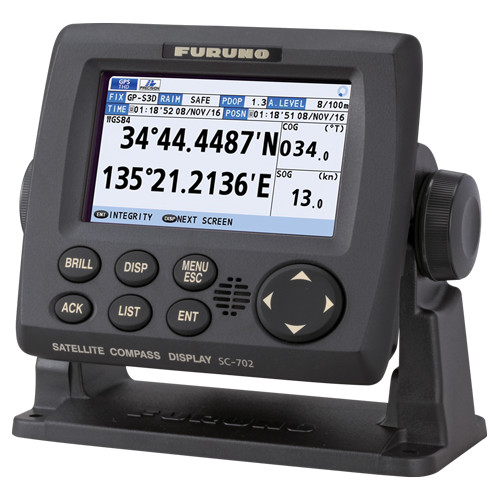
\includegraphics[width = 0.5\textwidth]{graphics/Furuno SC70.jpg}
	\caption{Furuno SC70. Differential GPS (DGPS) and compass}
	\label{fig:Furuno_SC70}
\end{figure}
Assuming normal noise distribution the measurement equations can be written as

\begin{align}
	HDT & = \psi + w                                    \\
	Pos & = \begin{bmatrix} x \\ y \end{bmatrix} + w              \\
	SoG & = \left|\begin{bmatrix} u \\ v \end{bmatrix}\right| + w \\
	CoG & = atan2(v,u) + w                              \\
	RoT & = r + w
\end{align}

\begin{align}
	\bm{y}   & = \bm{C}_m \bm{x} \\
	\bm{C}_m & = \bm{I}
\end{align}

\section{Control}
\begin{figure}[H]
	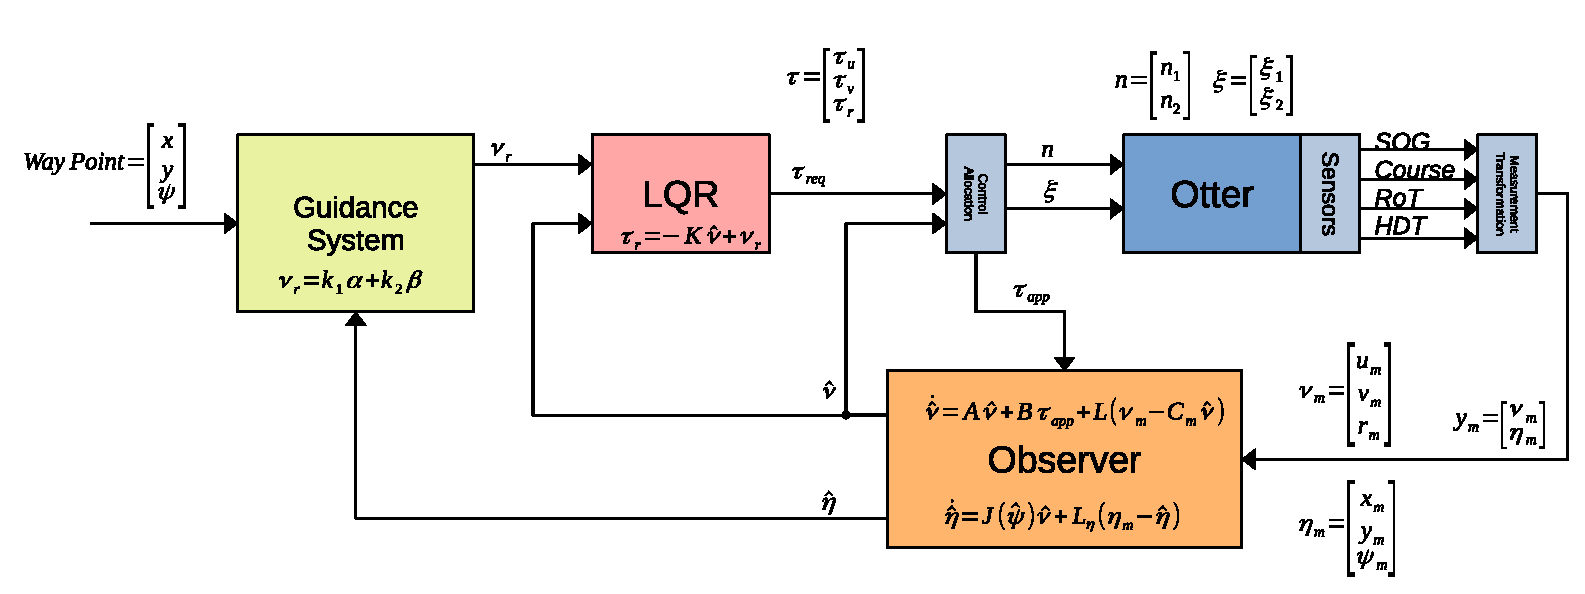
\includegraphics[width = \textwidth]{graphics/BlokDiagram.eps}
	\caption{}
	\label{}
\end{figure}

\end{document}
